
%----------------------------------------------------------------------------------------
%	Lecture 2
%----------------------------------------------------------------------------------------

\chapter{Vectors and Cross Product}  

\bigbreak
\section{Cross Product}

\subsection{Finding Area of A Triangle}

\begin{figure}[ht!]
    \centering
    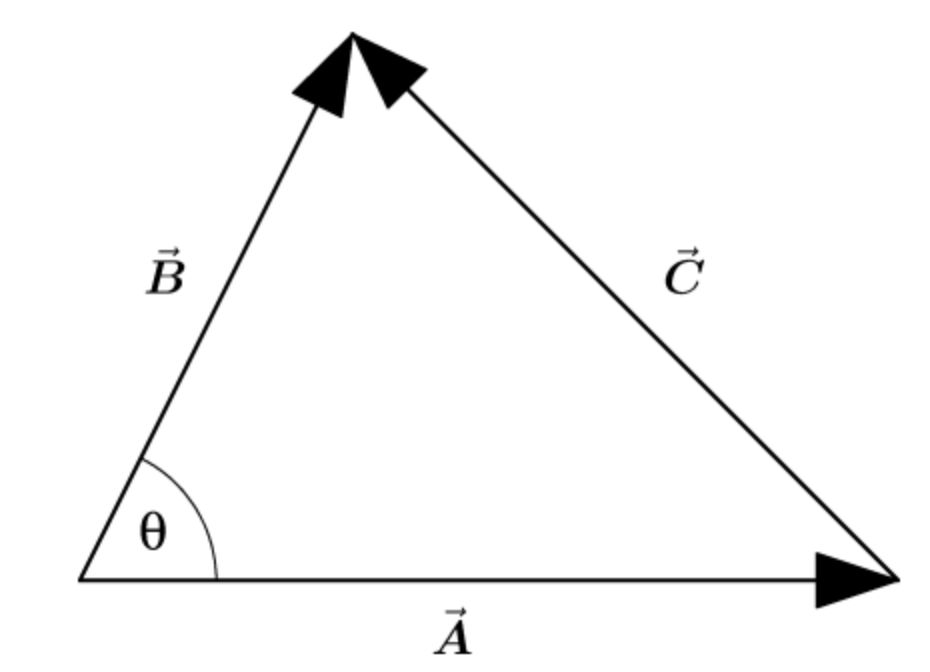
\includegraphics[scale=0.5]{./images/lecture_2_figure_1.png}
    \caption{Finding Area of a Triangle}
\end{figure}

We know that the area of a triangle is \ilds{ \frac{1}{2}(base)*(height) }.
And the $height = |{\bf B}| \sin \theta$. 
Thus, area of the triangle is \ilds{ \frac{1}{2} |{\bf A}| |{\bf B}| \sin \theta }.
Now, let us rotate {\bf A} to get ${\bf A'}$ so now the angle between ${\bf A'}$ and ${\bf B}$ is $90^{\circ} - \theta$.
Thus, the area of the triangle can be given as \ilds{\frac{1}{2} {\bf A'} \cdot {\bf B} } because $ \sin(\theta) = \cos(90^{\circ} - \theta) $

Let's say that that ${\bf A} = \ij{a_1}{a_2}$. Then we can say that ${\bf A'} = \ij{-a_2}{a_1}$.
Thus, area of the triangle is \ilds{\frac{1}{2}(-a_2 b_1 + a_1 b_2)}.
We can write is as 
\ilds{
    \frac{1}{2} 
    \begin{vmatrix*}
        a_1 & a_2 \\
        b_1 & b_2 \\
    \end{vmatrix*}
= \frac{1}{2}det({\bf A}, {\bf B})}.

The determinant measures the area of the paralellogram defined by vectors ${\bf A}$ and ${\bf B}$. 
So for the are of the triangle we divide it by half.
The determinant could be positive of the negative so for the area we need to take the absolute value of the determinant.

\subsection{Determinant in Space}

In three dimentions,
$$
det({\bf A}, {\bf B}, {\bf C}) = 
\begin{vmatrix*}
    a_1 & a_2 & a_3 \\
    b_1 & b_2 & b_3 \\
    c_1 & c_2 & c_3 
\end{vmatrix*}
$$

Geometrically, $det({\bf A}, {\bf B}, {\bf C}) = \pm \text{Volume of the parallelopiped}$.

\subsection{Definition of Cross Product}

{\bf Definition : } ${\bf A} \times {\bf B}$ is a vector given by the formula below.
$$
{\bf A} \times {\bf B} = 
\begin{vmatrix*}
    \hat{i} & \hat{j} & \hat{k} \\
    a_1 & a_2 & a_3 \\
    b_1 & b_2 & b_3
\end{vmatrix*}
$$

What is the geometric meaning of the cross product?


{\bf Theorem : } $|{\bf A} \times {\bf B}| = $ area of the paralellogram formed by ${\bf A}$ and  ${\bf B}$.
Direction of ${\bf A} \times {\bf B}$ is perpendicular to the plane of the paralellogram.


{\bf Right Hand Rule: } The direction of the of the cross product can be determinined by the right hand rule. 
Take your right hand and place your fingers along the vector ${\bf A}$ and then curl your fingers towards ${\bf B}$ using the smallest angle.
The direction of your thumb will show you the direction of their cross product.

General Rules :
\begin{enumerate}
    \item $\hat{i} \times \hat{j} = \hat{k}; \hat{j} \times \hat{k} = \hat{i}; \hat{k} \times \hat{i} = \hat{j}$ 
    \item ${\bf A} \times {\bf B} = - {\bf B} \times {\bf A}$
    \item $\hat{j} \times \hat{i} = - \hat{k}; \hat{k} \times \hat{j} = - \hat{i}; \hat{i} \times \hat{k} = - \hat{j}$  
\end{enumerate}

The above rules can be proven using the determinant definition.

\subsection{Another Look at Volume of Paralellopiped}

We can get the height of the parallelopiped by taking the component of the third vector along the normal vector of the base.

\begin{align*}
\text{Volume} &= (height) * (area of base) \\
    & = ({\bf A} \cdot \hat{n}) * (|{\bf B} \times {\bf C}|) )
\end{align*}
Here, $\hat{n}$ is the component of ${\bf A}$ along the vector ${\bf B} \times {\bf C}$.
So we can get $\hat{n}$ by \ilds{\hat{n} = \frac{{\bf B} \times {\bf C}}{|{\bf B} \times {\bf C}|} }
So, $$ \text{Volume} =  {\bf A} \cdot ({\bf B} \times {\bf C}) $$
We can verify that this triple product is the same as the determinant above.